% made by Gijs Groote on 18-07-2023

\documentclass{article}
\usepackage[utf8]{inputenc}

\usepackage{float}
\usepackage{caption}

\RequirePackage{tabularx}

\usepackage[table]{xcolor} 
\definecolor{myblue}{HTML}{CCF4FF}
\definecolor{myorange}{HTML}{FCAD68}

\usepackage{tikz}
\tikzstyle{decision} = [diamond, draw, fill=myblue, text width=4.5em, text badly centered, node distance=2.5cm, inner sep=0pt]
\tikzstyle{block} = [rectangle, draw, fill=myblue, align=center, rounded corners, minimum width = 2cm, minimum height=1cm]
\tikzstyle{line} = [draw, -latex']

\let\oldtextit\textit
\renewcommand{\textit}[1]{\Large{\oldtextit{#1}}}

\begin{document}
\pagestyle{empty}
\large

\section*{\hspace{-1cm}\Huge Metaal Laser - Workflow\vspace{0.7cm}}

TODO: Dit is van 3D printers!, Maak het voor de kunsstof laser!

\scalebox{1.3}{%
  \centering
  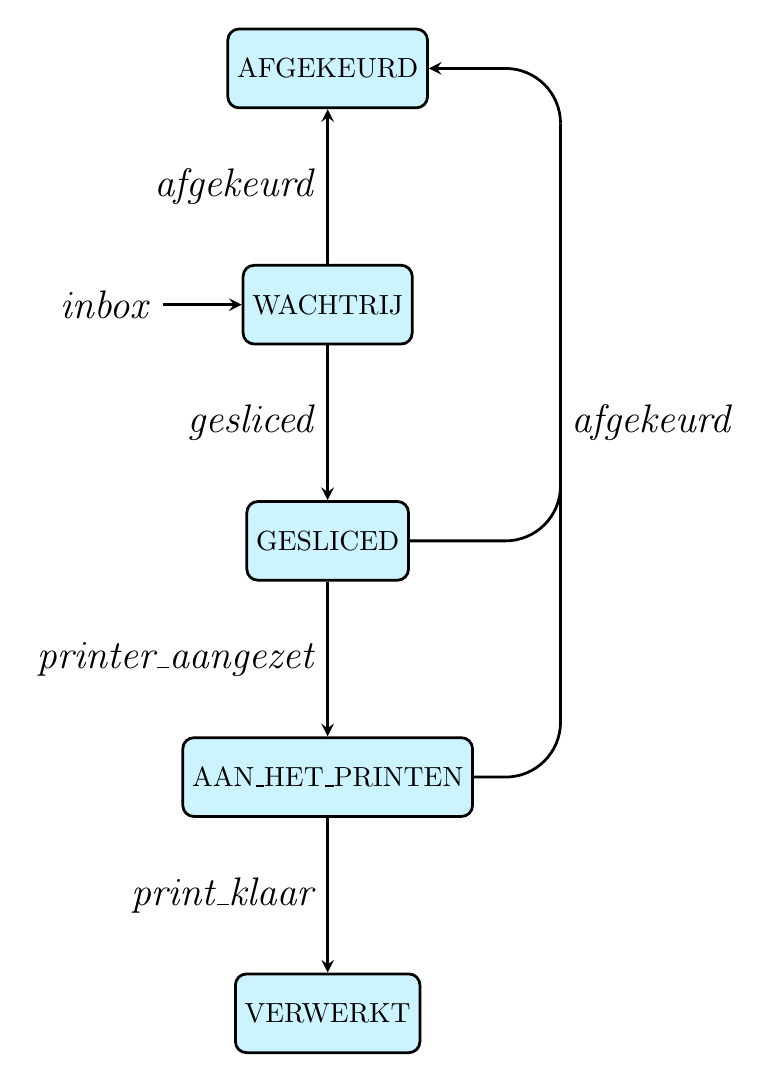
\begin{tikzpicture}[node distance = 3.0cm, line width=1pt]
    % Nodes
    \node [block] (wachtrij) {WACHTRIJ};
    \node [block, above of=wachtrij]  (afgekeurd) {AFGEKEURD};
    \node [block, below of=wachtrij]  (gesliced) {GESLICED};
    \node [block, below of=gesliced]  (aan_het_printen) {AAN\_HET\_PRINTEN};
    \node [block, below of=aan_het_printen] (verwerkt) {VERWERKT};

    % define lengths
    \pgfmathsetlengthmacro{\alpha}{0.7cm} % curve radius
    \pgfmathsetlengthmacro{\negalpha}{-\alpha}
    \pgfmathsetlengthmacro{\beta}{0.4cm} % straight bit before the curve

    % arrows
    \draw[>=stealth, ->, line width=1.0pt] ([xshift=-1.0cm]wachtrij.west) to node[xshift=-0.5cm,left]{\textit{inbox}} (wachtrij.west);
    \draw[>=stealth, ->, line width=1.0pt] (wachtrij.north) to node[left] {\textit{afgekeurd}} (afgekeurd.south);
    \draw[>=stealth, ->, line width=1.0pt] (wachtrij.south) to node[left] {\textit{gesliced}} (gesliced.north);
    \draw[>=stealth, -, line width=1.0pt] (aan_het_printen.east) -- ++(\beta,0)  to[out=0, in=-90] ++(\alpha, \alpha) -- node[right]{\textit{afgekeurd}} ([xshift=\alpha+\beta,yshift=\negalpha]afgekeurd.east -| aan_het_printen.east);
    \draw[>=stealth, <-, line width=1.0pt] (afgekeurd.east) -- ([xshift=\beta] afgekeurd -| aan_het_printen.east)  to[out=0, in=90] ++(\alpha,\negalpha);
    \draw[>=stealth, -, line width=1.0pt] (gesliced.east) -- ([xshift=\beta] gesliced -| aan_het_printen.east) to[out=0, in=-90] ++(\alpha,\alpha);
    \draw[>=stealth, ->, line width=1.0pt] (gesliced.south) to node[left] {\textit{printer\_aangezet}} (aan_het_printen.north);
    \draw[>=stealth, ->, line width=1.0pt] (aan_het_printen.south) to node[left] {\textit{print\_klaar}} (verwerkt.north);

  \end{tikzpicture}
}

\end{document}
